\section{Symbolic Execution}
Symbolic execution is method how to analyse a program. First researchs in this area were done around 1975. One of its main goals is to find certain programming errors, another possible goal is to prove that two programs handle each input exactly the same way. As you can image both of this problems are non trivial. In this publication the focus is on finding programming errors and other parts of symbolic execution might get pointed out, but will not be discussed in detail. 

Symbolic execution focuses on problems that can not be determined by static code analysis, because they require the execution of the program. In contradiction to a normal execution, for example in manual unit tests, random fuzzing or even actual user input, this analysis uses so called symbolic input.

In contrast to a variable with a concrete value, for example 5, a variable with a symbolic value can have any value. This symbolic value will get certain restrictions during the execution of the program. During the execution of the program the execution engine will track all assigned variables. This collection of variables is called symbolic memory store and $\sigma$ will be used to denote it in mathematical terms.\cite{SurveySymExec-CSUR18}.
Whenever a variable gets a new value, the variable and its value will be added to the memory store. If the variable is based on a variable with a symbolic value then the new variable will also get a symbolic value. If its based on a conrecte value then the concrete value itself will be stored.

Consider the following example where the variables a and b are symbolic and the according values denoted with the symbols $\alpha_a$ and $\alpha_b$:
$$\sigma = \{a\gets \alpha_a , b \gets \alpha_b\}$$
If we assign a new variable c = 2*a the memory store will be updated to include c and thus be
$$\sigma = \{a\gets \alpha_a , b \gets \alpha_b, c \gets 2*\alpha_a\}$$
If we assign the value $1$ to the variable a $a = 1$ then the memory store will get updated too. Note that the symbolic value $\alpha_a$ stays in the variable c, as this assignment has been made before the variable $a$ got a new value.
$$\sigma = \{a\gets 1, b \gets \alpha_b, c \gets 2*\alpha_a\}$$


Whenever a branching statement\footnote{For example the if-statement or switch-statement} is reached that depends on a symbolic value, the symbolic execution engine must follow both of the branches and restrict the symbolic value in regard to the condition. These restrictions are collected and together describe all conditions that the symbolic variables must satisfy in this specific branch. This collection is often called path condition or path constraints and $\pi$ used to denote it\cite{SurveySymExec-CSUR18}.
Consider for example that a statement $if (a > 0)$ is the first statement of your code. Because this is a branching statement the execution engine has to calucate two different path constraints $\pi_{true}$ and $\pi_{false}$
$$\pi_{true} = \alpha_a = 0$$
$$\pi_{false} = \alpha_a <= 0$$

Directly after the branching the path condition can be handed to an SMT solver, which will try to find concrete values to all the variables in the symbolic memory store, so that the condition is satisfied. If the SMT solver decides that a condition is not satisfiable this path of the pogram does not need further research, as it can no be reached.

\begin{codesnippet}[caption={Simple Symbolic Execution Example}, label={codeSnippetSymbolicExecution}]
int calculateMagicNumber(int a, int b){
   int x = 1;
   if(a >= 0){
      if (b > 0){
         a = a + x;
      }
      if(b < 0){
        a = a*b;
      }
   }else{
     a = a*-1;
   }
  assert(a != 0);
  return a * b
}
\end{codesnippet}

\begin {figure*}%[!hbtp]
\begin{adjustbox}{width=\textwidth}
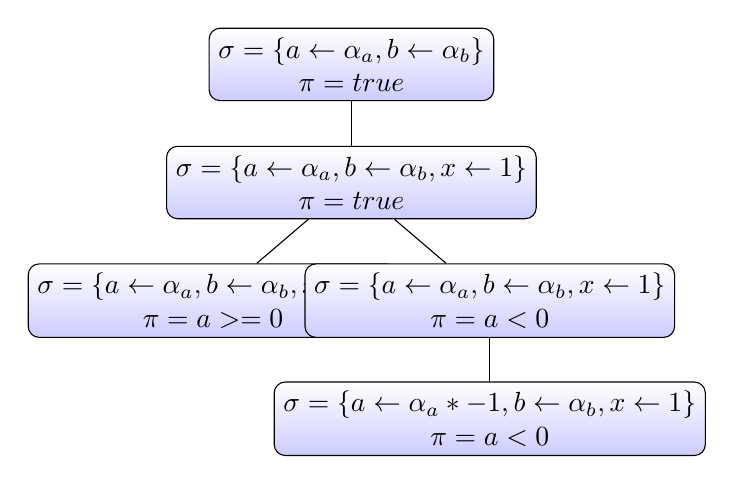
\begin{tikzpicture}[sibling distance=10em,
  every node/.style = {shape=rectangle, rounded corners,
    draw, align=center,
    top color=white, bottom color=blue!20}]]
  \node {$\sigma = \{a\gets \alpha_a , b \gets \alpha_b\}$\\$\pi = true$}
    child { node {$\sigma = \{a\gets \alpha_a , b \gets \alpha_b, x \gets 1\}$\\$\pi = true$}
	child { node {$\sigma = \{a\gets \alpha_a , b \gets \alpha_b, x \gets 1\}$\\$\pi = a>=0$}}
	child { node {$\sigma = \{a\gets \alpha_a , b \gets \alpha_b, x \gets 1\}$\\$\pi = a<0$}
		child { node {$\sigma = \{a\gets \alpha_a*-1 , b \gets \alpha_b, x \gets 1\}$\\$\pi = a<0$}}
}}

;
\end{tikzpicture}
\end{adjustbox}
\end{figure*}





Introduction to the topic of symbolic execution and its limits \cite{SurveySymExec-CSUR18} . Information about symbolic execution is also included in nearly all sources listed in the section concolic testing\todo{Cleanup}